% Plantilla comprimida UC3M + ISCIII, para documentos con muy poco espacio
% (resumenes a una cara, entregas cortas, etc.). Demo de titulo minimo con
% fila de logos, secciones compactas (con subsubseccion en formato
% "run-in"), lista, tabla y figura.
% Version a UNA columna: un resumen corto, con demo de bibliografia
% (bibtex) y su seccion de referencias al final. El cuerpo por si solo cabe
% en una cara; las dos referencias de ejemplo empujan un par de lineas a
% una segunda pagina, que es justo lo esperable con contenido real en un
% documento pensado para muy poco espacio. Ver main-twocolumn.tex para el
% mismo paquete a dos columnas, con mas contenido (el caso de uso real de
% dos columnas es tener mas texto del que cabria en una sola).
%
% Compilar:  make      (latexmk -lualatex, genera build/main.pdf y
%                        build/main-twocolumn.pdf)
%
% No hace falta cargar inputenc ni fontenc: bajo LuaLaTeX+fontspec la
% codificacion la gestiona el motor.
\documentclass[10pt]{article}

% babel va ANTES que uc3misciitight: el paquete carga hyperref internamente,
% y hyperref necesita que babel este ya activo para traducir al espanol los
% nombres que genera \autoref.
\usepackage[spanish,es-noquoting]{babel}
\usepackage{uc3misciitight}

\title{Resumen: caché de resultados en la capa de consultas}
\subject{Bases de Datos}
\group{Grupo 84}
\author{Raúl Aguilar Arroyo \and Ana Pérez Ruiz}
\date{Curso 2026/2027}

\begin{document}
\maketitle

\section{Motivación}

El coste de recalcular consultas repetidas sobre el mismo conjunto de datos
motiva introducir una capa de caché entre la aplicación y el motor de base
de datos, reduciendo la latencia percibida sin modificar el esquema
subyacente.

\subsection{Planteamiento}

Se evalúa una caché LRU en memoria situada delante del motor
relacional~\cite{megiddo2003}, invalidada de forma explícita en cada
escritura sobre las tablas afectadas~\cite{silberschatz2019}.

\subsubsection{Alcance} Este resumen cubre únicamente el caso de consultas
de solo lectura sobre una única tabla; los joins multi-tabla quedan fuera
del análisis presentado aquí.

\section{Resultados}

La \autoref{tab:resultados} resume la reducción de latencia observada para
distintos tamaños de caché.

\begin{table}[h]
  \centering
  \caption{Latencia media según tamaño de caché.}
  \label{tab:resultados}
  \begin{tabular}{@{}lrr@{}}
    \toprule
    Tamaño caché & Latencia (ms) & Aciertos (\%) \\
    \midrule
    Sin caché & 42 & --- \\
    128 entradas & 19 & 61 \\
    512 entradas & 8 & 89 \\
    \bottomrule
  \end{tabular}
\end{table}

Ventajas observadas:
\begin{itemize}
  \item Reducción de latencia media superior al 80\,\% con 512 entradas.
  \item Sin cambios en el esquema ni en las consultas de la aplicación.
\end{itemize}

La \autoref{fig:latencia} ilustra la tendencia.

\begin{figure}[h]
  \centering
  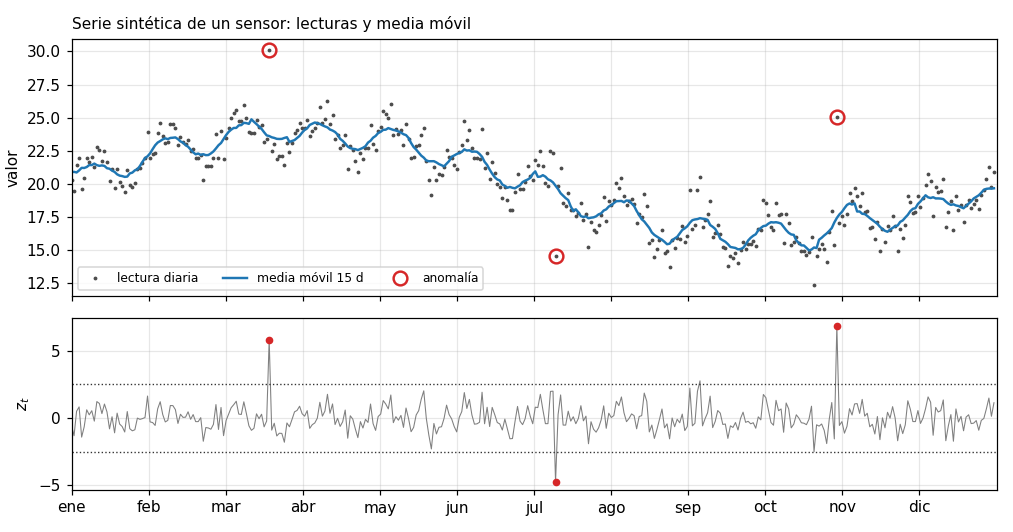
\includegraphics[width=\linewidth]{figs/demo-figura}
  \caption{Latencia media en función del tamaño de la caché.}
  \label{fig:latencia}
\end{figure}

\section{Conclusión}

Una caché LRU sencilla, invalidada por escritura, ofrece una reducción de
latencia sustancial con una complejidad de implementación baja, siempre que
las consultas se limiten a lecturas de una sola tabla.

\bibliographystyle{plain}
\bibliography{referencias}

\end{document}
